% =============================================================================
% FAECO 中文期刊版式（计算机辅助设计与图形学学报模板近似）
% 字体说明：模板要求方正书宋_GBK/方正仿宋_GBK/黑体/Times New Roman。
% 方正 GBK 字库为商业字体，需作者自行购买安装；当前以系统宋体/黑体/仿宋近似。
% 安装方正字库后，将下方 FZ 字体变量替换为对应方正字体名即可。
% =============================================================================
\documentclass[twocolumn,10pt,fontset=windows]{ctexart}

% -----------------------------------------------------------------------------
% 字体（方正 GBK 安装后替换此处）
%   正文:    \setCJKmainfont{方正书宋_GBK}
%   标题:    \setCJKsansfont{方正黑体_GBK}
%   仿宋:    \setCJKfamilyfont{fzfs}{方正仿宋_GBK}
% 当前用系统字体近似（fontset=windows: 宋体/黑体/楷体/仿宋）
% -----------------------------------------------------------------------------
\setmainfont[Path=./fonts/,Extension=.ttf,UprightFont=times,BoldFont=timesbd,ItalicFont=timesi,BoldItalicFont=timesbi]{Times New Roman}
\setCJKmainfont[Path=./fonts/,Extension=.ttf]{FZShuSong-Z01}
\setCJKsansfont[Path=./fonts/,Extension=.ttf]{SimHei}
\newCJKfontfamily\songfamily[Path=./fonts/,Extension=.ttf]{FZShuSong-Z01}
\newCJKfontfamily\fangfamily[Path=./fonts/,Extension=.ttf]{FZFangSong-Z02}
\newCJKfontfamily\heifamily[Path=./fonts/,Extension=.ttf]{SimHei}
\usepackage{amsmath,amssymb}
\usepackage{newtxmath}
\let\songti\songfamily\let\heiti\heifamily\let\fangsong\fangfamily
\usepackage{booktabs}
\usepackage{graphicx}
\usepackage{subfig}
\usepackage{float}
\usepackage{array}
\usepackage[nocompress]{cite}
\usepackage[hidelinks]{hyperref}
\usepackage{xurl}
\usepackage{algorithm}
\usepackage{algpseudocode}
\usepackage{multirow}
\usepackage{geometry}
\usepackage{placeins}
\usepackage{dblfloatfix}
\usepackage{balance}

% 版面：A4 双栏，栏宽 21.59 字符、栏间距 3 字符（以 3zw 近似）
\geometry{a4paper,left=2.0cm,right=2.0cm,top=2.1cm,bottom=2.1cm,columnsep=31.5pt}

\renewcommand{\eqref}[1]{\textup{（\ref{#1}）}}
\graphicspath{{../figures/}}
\setlength{\emergencystretch}{3em}
\Urlmuskip=0mu plus 3mu\relax
\raggedbottom
\setlength{\floatsep}{6pt plus 2pt minus 2pt}
\setlength{\textfloatsep}{8pt plus 2pt minus 2pt}
\setlength{\intextsep}{6pt plus 2pt minus 2pt}
\setlength{\dblfloatsep}{6pt plus 2pt minus 2pt}
\setlength{\dbltextfloatsep}{8pt plus 2pt minus 2pt}

% -----------------------------------------------------------------------------
% 标题层级（模板：1级11.5pt黑体 / 2级五号黑体 / 3级10pt书宋）
% -----------------------------------------------------------------------------
\ctexset{
  section = {format=\heiti\fontsize{11.5}{15}\selectfont, beforeskip=6pt, afterskip=4pt},
  subsection = {format=\heiti\fontsize{10.5}{14}\selectfont, beforeskip=5pt, afterskip=3pt},
  subsubsection = {format=\songti\fontsize{10}{13}\selectfont, beforeskip=4pt, afterskip=2pt}
}

% 图题（书宋9pt）、表题（黑体9pt）、表注/分图题（书宋8pt）
\usepackage{caption}
\DeclareCaptionFont{songti}{\songti}
\DeclareCaptionFont{heiti}{\heiti}
\captionsetup[figure]{font={songti,small},labelfont={bf},skip=3pt}
\captionsetup[table]{font={heiti,small},labelfont={bf},skip=3pt}
% subfig is not used in this manuscript; do not configure an unused subfloat caption.
\captionsetup{labelsep=space}

\begin{document}

\pagestyle{plain}

% -----------------------------------------------------------------------------
% 中文首部：标题/作者/单位/摘要/关键词/中图法分类号/DOI
\twocolumn[
\vspace*{-0.25cm}
\begin{center}
{\heiti\zihao{3} FAECO：面向预布局门级时序 ECO 的失效驱动候选搜索}\par
\vspace{6pt}
{\fangsong\zihao{4} 佟亚龙、刘畅}\par
\vspace{4pt}
{\songti\fontsize{8}{12}\selectfont（国防科技大学计算机学院，长沙 410073）}\par\vspace{2pt}
{\songti\fontsize{8}{12}\selectfont E-mail：chancews@qq.com（通信作者）}\par
\vspace{6pt}
\end{center}
\begin{flushleft}
  {\heiti\fontsize{8.5}{13}\selectfont 摘\quad 要：}{\songti\fontsize{8.5}{13}\selectfont 针对预布局门级时序 ECO 中缓冲器插入和门尺寸调整难以压缩深层逻辑的问题，本文提出失效驱动候选搜索引擎（Failure-Aware ECO，FAECO）。该方法在已映射网表的违例扇入锥上构造多特征加权割，将局部功能保持候选的可用性、关键路径覆盖和候选规模编码为割权重，并根据候选失败类型更新后续搜索。候选先经库函数和结构规则筛选，再由 OpenSTA 在理想线网模式下测量时序收益；满足条件的候选进入基于标准寄生交换格式（SPEF）的简化复测。在三组测试集上，FAECO 分别实现 8/8、19/19 和 2/3 个电路的严格 WNS 改善；ITC-99 全部 19 个电路均无回退。独立逻辑门级顺序 SEC 对最终基线网表与修复网表分别实现 8/8、19/19 和 3/3 通过。收敛配置下混合策略平均改善不为负，真实布局布线后 5/8 个电路保持改善。}
\par
\vspace{4pt}
{\heiti\fontsize{8.5}{13}\selectfont 关键词：}{\songti\fontsize{8.5}{13}\selectfont 时序 ECO；门级局部重构；多特征加权割；失效驱动反馈；简化 SPEF 门控；预布局时序优化}\par
\vspace{2pt}
{\songti\fontsize{8.5}{13}\selectfont 中图法分类号：TP391.41}\par
\vspace{2pt}
{\songti\fontsize{8.5}{13}\selectfont DOI：未分配}
\end{flushleft}
\vspace{4pt}
% 英文题录
\begin{center}
{\bfseries\fontsize{13.5}{18}\selectfont FAECO: Failure-Aware Candidate Search for Pre-Placement Gate-Level Timing ECO}\par
\vspace{3pt}
{\normalsize Tong Yalong, Liu Chang\par}
\vspace{3pt}
{\small \itshape (College of Computer Science, National University of Defense Technology, Changsha 410073, China)}\par
\vspace{4pt}
\end{center}
\begin{flushleft}
  {\bfseries Abstract:} {\small We present Failure-Aware ECO (FAECO), a failure-aware candidate-search engine for pre-placement gate-level timing ECO, to address the limited ability of buffer insertion and gate sizing to compress deep logic. FAECO constructs a multi-feature weighted cut over violating fan-in cones of mapped netlists, encoding local function-preservation availability, critical-path coverage, and candidate size, and updates the search through candidate failures; candidates are screened by library-function and structural rules, accepted by OpenSTA measurements on ideal nets, and subjected to simplified rechecking using SPEF. Across three benchmark sets, FAECO achieves strict WNS improvement on 8/8, 19/19, and 2/3 circuits, respectively; the ITC-99 suite has no regression. Independent logical gate-level SEC passes all reported baseline--repair pairs: 8/8 ISCAS89, 19/19 ITC-99, and 3/3 PicoRV32. Under the convergence configuration, the mixed strategy achieves a non-negative mean improvement across all suites, and 5/8 ISCAS89 circuits retain an improvement after real placement and routing.}\par
\vspace{3pt}
{\bfseries Key words:} {\small gate-level timing ECO; local restructuring; multi-feature weighted cut; failure-aware feedback; simplified SPEF gate; pre-placement timing optimization}\par
\end{flushleft}
]%


% =============================================================================
% I. 引言
% =============================================================================
\section{引言}

\subsection{背景与问题}
工程变更命令（engineering change order，ECO）按修复目标可分为功能 ECO 与时序 ECO：前者修复逻辑功能错误，后者修复时序违例。本文聚焦综合后、布局布线前的门级时序 ECO。本文将“局部重构”定义为在已映射网表的违例扇入锥上执行等价单元替换、门尺寸调整、缓冲器插入和少量多门组合，完整的寄存器传输级（register-transfer level，RTL）综合属于上游网表生成阶段。传统时序 ECO 主要依赖缓冲器插入（buffer insertion，B）与门尺寸调整（gate sizing，G），通过调整单元延迟修复最差负松弛（worst negative slack，WNS）与总负松弛（total negative slack，TNS）。在严重路径违例下，B/G 优化能力不足，其结构重映射仍受候选空间限制\cite{ho2010eco,liu2021rlsizer,chen2024aito}。

工业实践中，将违例锥（最差负松弛路径所在的扇入逻辑锥）整体替换为时序友好补丁的做法比 B/G 更稳定，但通常依赖工业数据。逻辑补丁构造与物理优化的协同关系直接影响功能等价验证和时序收益；两者失配时，补丁替换收敛缓慢甚至失败。

上述方法留下三个需要在公开工具链上量化的问题：第一，候选构造阶段的功能保持偏好对无效候选数量的影响；第二，理想线网时序收益与线载变化之间的筛选关系；第三，候选失败信息对下一轮搜索空间的收缩作用。
\subsection{研究动机}
本文的研究动机是扩大预布局门级时序 ECO 的局部结构搜索空间，同时让候选验证和物理复测保持在可控成本内。为此，FAECO 在已映射网表的违例扇入锥上构造多特征加权割，将局部功能保持能力、关键路径覆盖和候选规模纳入候选排序，并把候选失败类型转化为下一轮搜索的反馈信号。

实验范围限定为已映射门级网表和公开的 SKY130 HD 标准单元库。主实验采用 ISCAS89 顺序电路基准集\cite{iscas89}；跨测试集实验采用能够在相同流程下映射到 SKY130 HD 的 ITC-99 电路\cite{itc99}，并加入 PicoRV32 的三个结构不同子模块\cite{picorv32}。时序收益由理想线网 STA 筛选，再用简化 SPEF 复测；最终基线网表与修复网表通过独立顺序 SEC 检查。

\subsection{主要贡献}
本文的主要贡献体现为以下三个亮点：

\begin{enumerate}
  \item \textbf{失效驱动搜索}：以局部功能保持能力、关键路径覆盖和候选规模构造多特征加权割，并用 F1--F6 失败反馈更新割权重与搜索顺序，形成面向深层逻辑的闭环候选生成机制。
  \item \textbf{功能—时序—物理分层验证}：将局部函数/结构筛选、理想线网 WNS 判定和简化 SPEF 复测串联起来，并以独立全网表 SEC 验证最终修复结果；三组测试集的最终基线—修复网表均通过独立顺序 SEC（30/30）。
  \item \textbf{跨测试集与真实流程验证}：在 ISCAS89、ITC-99 和 PicoRV32 上分别实现 8/8、19/19 和 2/3 个电路的严格 WNS 改善；收敛配置下混合策略平均改善不为负，真实布局布线后 8 个 ISCAS89 电路中有 5 个保持改善。
\end{enumerate}

% =============================================================================
% II. 相关工作
% =============================================================================
\section{相关工作}

\subsection{结构重映射与逻辑补丁}
ECO 修复主要分为三类技术路径：基于备用单元的结构重映射、基于逻辑补丁构造的功能修复，以及基于缓冲器插入与门尺寸调整的物理优化。

结构重映射以缓冲插入、尺寸调整与技术重映射的流程修复时序，将布线代价纳入备用单元分配\cite{ho2010eco}，或以符号采样搜索修正点\cite{kravets2019symbolic}。代表性流程通常先构造候选，再由等价性或时序验证筛选；FAECO 将可计算的局部功能保持候选可用性前置到候选构造阶段，全局顺序等价性检查（sequential equivalence checking，SEC）作为独立验证环节。例如，\cite{ho2010eco}的备用单元分配以布线后负载为输入，FAECO 则在预布局阶段完成候选构造；\cite{kravets2019symbolic}的符号采样扩大搜索范围，并通过验证结果筛选修正点。

逻辑补丁构造通常先沿违例路径切分扇入逻辑锥，提取局部窗口；随后利用功能约简与反相器图（functionally reduced and-inverter graph，FRAIG）表示候选逻辑，再通过 SAT 证明筛选与原逻辑功能等价的补丁，以修复功能错误\cite{jiang2010fraig,jiang2016resource}。

后续工作进一步将资源代价纳入补丁生成，并采用 SAT 或组合等价性检查（combinational equivalence checking，CEC）进行复核\cite{jiang2016resource,zhong2024stp}。FAECO 将可计算的局部功能保持信息提前用于候选排序，并把理想线网时序测量作为独立接受信号。

当等价性验证失败时，代表性流程通常需要扩大搜索窗口或增加补丁规模重新枚举\cite{zhuo2018patch}；在数十万门级设计上，这一过程会增加计算开销和收敛成本。

B/G 物理优化近年来主要沿门尺寸调整、联合 B/G 和物理感知方向发展\cite{liu2021rlsizer,huang2025phys,chen2024aito,zhang2025buffalo}；这些方法保持逻辑结构不变，主要覆盖路径级负载优化；FAECO 进一步面向逻辑级数和关键路径结构进行局部重构。

学习驱动方法\cite{chen2024aito,zhang2025buffalo}提升了门尺寸调整和缓冲器优化效率，同时保持逻辑结构不变。

\subsection{B/G 物理优化与研究定位}
本文比较的若干方法依赖商用 EDA 引擎或内部工业流程；本文选择公开的 Yosys\cite{yosys}、OpenSTA\cite{opensta} 与 OpenROAD\cite{openroad}，在 SKY130 HD\cite{sky130} 上实现并评估门级候选搜索。FAECO 流程覆盖映射网表、候选生成、理想线网静态时序分析（STA）和布局布线后核验；顺序主实验采用构造级状态保持检查，独立的全网表 SEC 作为后续验证环节。

从应用阶段看，结构重映射与 B/G 物理优化面向后布局、后布线阶段的物理微调，逻辑补丁构造则多在综合后、布局前执行功能修复。FAECO 位于两者之间：在已映射网表上进行局部门级重构，同时用理想线网 STA 和简化线载模型进行预布局筛选。

上述四类方法的主要侧重点汇总如表~\ref{tab:related_diff}。

\begin{table}[ht]
\centering
\caption{四类方法的主要侧重点}
\label{tab:related_diff}
\footnotesize
\setlength{\tabcolsep}{2pt}
\begin{tabular}{>{\raggedright\arraybackslash}p{1.55cm}>{\raggedright\arraybackslash}p{2.55cm}>{\raggedright\arraybackslash}p{3.2cm}}
\toprule
\textbf{方法} & \textbf{主要优势} & \textbf{适用问题} \\
\midrule
结构重映射 & 改变局部逻辑拓扑 & 深层逻辑和结构性时序违例 \\
逻辑补丁 & 局部重构并支持 SAT/CEC 验证 & 功能 ECO 或功能—时序联合修复 \\
B/G 优化 & 利用驱动与负载信息进行物理微调 & 后布局的小幅时序违例 \\
FAECO & 加权割生成候选并按失败反馈迭代搜索 & 预布局已映射网表的深层逻辑时序 ECO \\
\bottomrule
\end{tabular}
\end{table}

\section{方法}

\subsection{问题定义与设计目标}
给定映射网表 $G'$、目标周期 $T$、时序约束和工艺库 $\mathcal{L}$，FAECO 在违例端点的扇入锥上搜索局部候选 $p$，得到修复网表 $G^*$。主实验以 $\Delta_{\mathrm{WNS}}(p)>0$ 作为接受条件，并要求修复前后网表保持功能等价；可选的 TNS 感知配置仅在 WNS 持平且 TNS 改善时接受候选。四类局部变换为：R（布尔函数等价替换）、G（驱动尺寸调整）、B（恒等缓冲器插入）和 JOINT（联合枚举）。顺序实验不修改 D 触发器、时钟或复位单元。

候选 $p$ 由局部门集合及其边界端口构成，且仅在不含三态、时钟门控和复位逻辑的组合局部上生成。候选构造使用库函数匹配和结构规则进行前置筛选，最终功能保持由独立顺序 SEC 验证。加权割构造见 \S\ref{sec:mechanism}，符号见表~\ref{tab:symbols}。

\begin{table}[ht]
\centering
\caption{符号表}
\label{tab:symbols}
\scriptsize
\setlength{\tabcolsep}{2pt}
\renewcommand{\arraystretch}{0.9}
\begin{tabular}{p{2.6cm}p{4.9cm}}
\toprule
\textbf{符号} & \textbf{定义} \\
\midrule
$G = (V, E)$ & 门级网图，顶点为门/端口，边为信号线 \\
$C(G, t) \subseteq V$ & 目标输出 $t$ 的扇入锥 \\
$K(G, t)$ & 由每个门的输入/输出容量边与扇入依赖边构成的 $s$-$t$ 分裂图 \\
$\mathrm{cost}(v)$ & 门 $v$ 的节点代价，见式~\eqref{eq:cost} \\
$s(v)$、$n_C=|C(G,t)|$、$S=\sum_u s(u)^2$ & 门 $v$ 的局部扇入锥规模、目标锥门数与锥内规模平方和 \\
$\lambda_b,\lambda_s,\lambda_v,\lambda_c,\lambda_f$ & 边界、尺寸、验证、关键覆盖与扇出等割图权重；$\lambda_c$ 用于关键路径覆盖候选的反馈 \\
$\mathrm{priority}(p)$ & 候选优先级，由加权割顺序、关键路径覆盖候选和策略优先级表共同确定 \\
F1--F6 & 六类失败类型，定义见表~\ref{tab:failures} \\
\bottomrule
\multicolumn{2}{p{7.3cm}}{\footnotesize 候选优先级决定测量顺序，候选接受由 OpenSTA 实测结果决定；F1--F6 反馈作用于下一轮的割权重更新。}\\
\end{tabular}
\end{table}

\subsection{方法总览}\label{sec:overview}

FAECO 包含映射准备、候选生成和时序验证三个阶段，如图~\ref{fig:method_flow} 所示。候选策略为 R、G、B 和 JOINT。

\begin{enumerate}
  \item[(a)] \textbf{映射准备}：经 Yosys 两步流程\cite{yosys}生成 SKY130 HD 映射网表 $G'$；Liberty 文件提供单元逻辑和时序信息\cite{liberty}，BLIF 归一化与 ABC \texttt{cec}\cite{abc} 用于组合网表回验。
  \item[(b)] \textbf{加权割与候选生成}：在扇入锥 $C(G,t)$ 上构建 s-t 分裂图。Liberty 函数匹配生成 R 候选集；无 R 候选的门降低关键路径奖励并转向 G/B。候选由加权最小割和关键路径覆盖割产生，按割代价、路径覆盖和策略优先级排序；OpenSTA 结果用于接受判定，F1--F6 反馈用于更新权重。
  \item[(c)] \textbf{验证与接受}：候选经库函数和结构规则筛选后，由 OpenSTA 在理想线网模式下测量 WNS/TNS；启用物理门控时，理想增益超过 10 ps 的候选进入简化 SPEF 复测。
\end{enumerate}

\begin{figure}[!t]
\centering
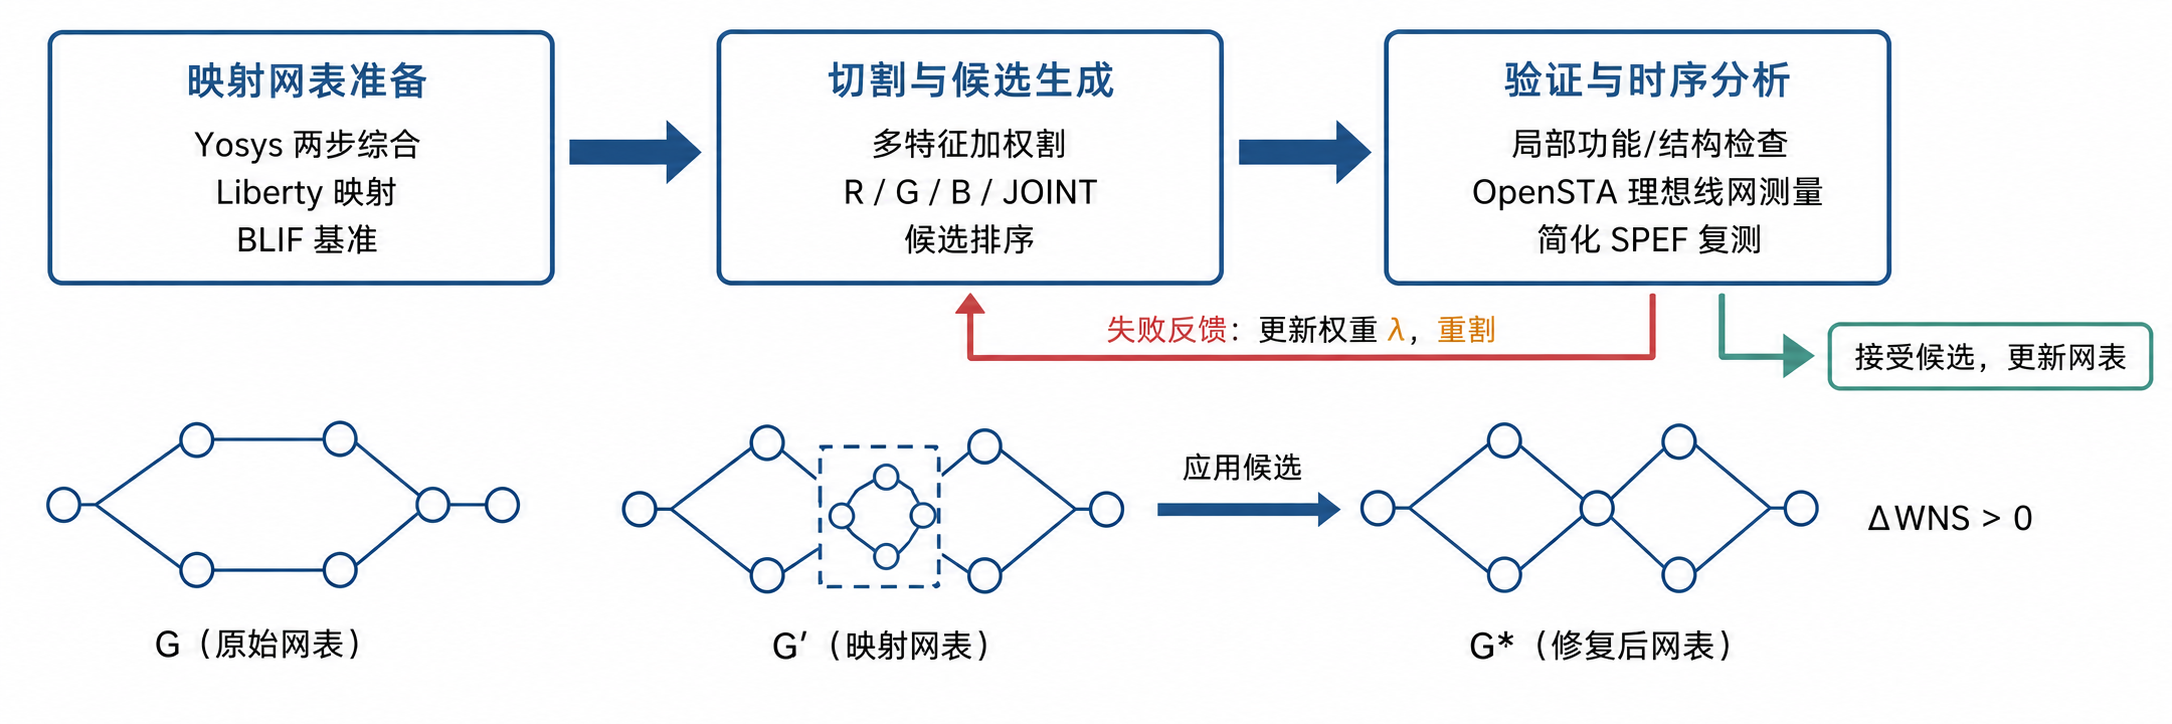
\includegraphics[width=0.96\columnwidth]{fig_method_flow_redraw_20260814.png}%
\caption{FAECO 三阶段流水线：映射网表准备 $\rightarrow$ 切割与候选细化 $\rightarrow$ 验证与时序分析。}
\label{fig:method_flow}
\end{figure}

\begin{algorithm}[!t]
\footnotesize
\caption{FAECO 修复流程示意}\label{alg:main}
\begin{algorithmic}[1]
\Require 映射网表 $G'$、时序约束 $T$、工艺库 $\mathcal{L}$
\Ensure 修复后网表 $G^*$、接受候选集合 $\mathcal{A}$
\State 保存基线网表 $G_0\gets G'$，初始化 $G^*\gets G_0$、$\mathcal{A}\gets\emptyset$ 和搜索权重 $\lambda$
\Repeat
  \State 从最差违例端点提取扇入锥，必要时按深度分治
  \State 构建加权割与关键路径覆盖割，生成并排序 R/G/B/JOINT 候选
  \State 对候选执行局部功能/结构检查和 OpenSTA 测量
  \State 对满足物理门控条件的候选进行简化 SPEF 复测
  \State 从 $G_0$ 应用满足条件的候选并得到 $G^*$，更新 $\mathcal{A}$；否则根据失败类型更新对应的 $\lambda$
\Until{无时序违例、候选耗尽或达到停止条件}
\State \Return $G^*,\ \mathcal{A}$
\end{algorithmic}
\end{algorithm}

算法~\ref{alg:main} 给出从违例端点提取扇入锥、生成候选、时序测量到反馈重搜索的流程。候选接受谓词和验证层次在 \S\ref{sec:validation} 中统一定义。

\subsection{多特征加权割与候选生成}\label{sec:mechanism}
\begin{figure*}[t]
\centering
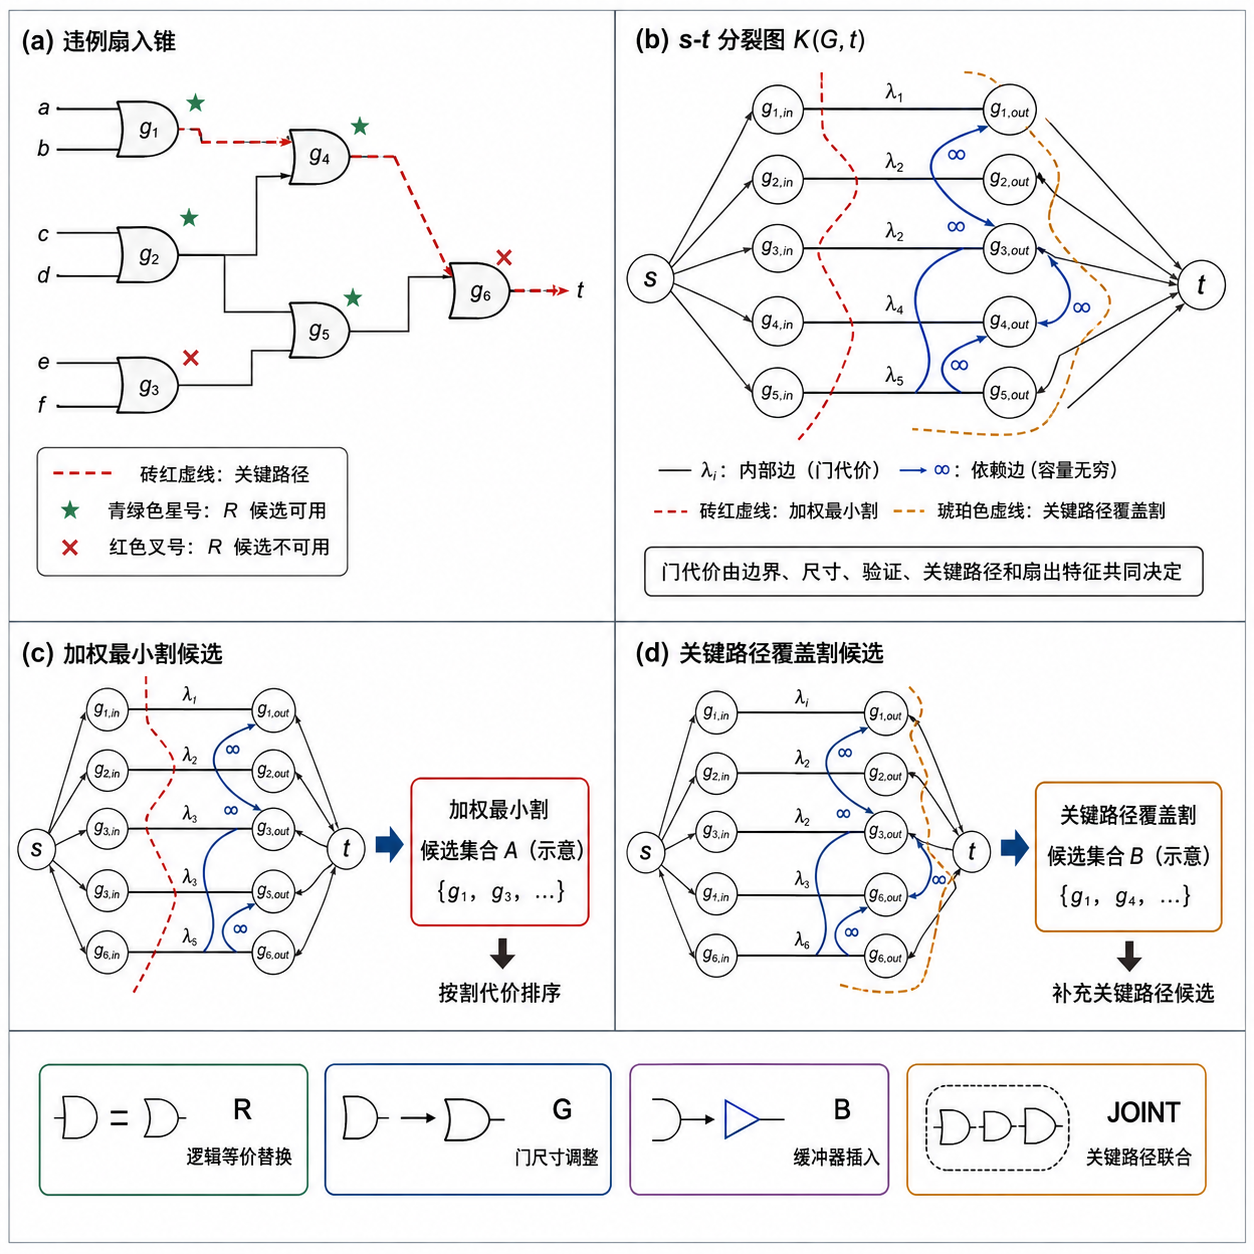
\includegraphics[width=0.98\textwidth]{fig_cut_generation_mechanism_imagegen.png}
\caption{FAECO 机制原理：局部扇入锥中的特征决定节点代价，节点代价决定割边界，割边界生成等价候选并由 OpenSTA 反馈更新。}
\label{fig:cut_generation}
\end{figure*}

图~\ref{fig:cut_generation} 展示 FAECO 的核心原理。首先，从违例端点反向提取局部组合扇入锥 $C(G,t)$，并为门节点标注功能保持可用性、关键路径覆盖和候选规模等特征。在 s-t 分裂图 $K(G,t)$ 中，这些特征共同写入节点代价：边界、尺寸、验证和扇出项控制候选规模，关键路径覆盖项提高关键门附近的代价权重，使割边界随特征变化而移动。

随后，FAECO 生成加权最小割和关键路径覆盖割两类互补边界：前者优先控制局部规模，后者覆盖时序关键门。两类边界分别形成候选集 A 和候选集 B，再实例化为 R/G/B/JOINT 候选，并交由 OpenSTA 测量 $\Delta_{\mathrm{WNS}}$ 和 $\Delta_{\mathrm{TNS}}$。接受谓词保留有效候选；失败候选根据失败类型反馈至割权重，驱动下一轮重割。

候选 $p$ 的 WNS 改善量在相同 SDC 和时钟约束下定义为：
\begin{equation}\label{eq:dtiming}
\Delta_{\mathrm{WNS}}(p) = \mathrm{WNS}_{\mathrm{after}}(p) - \mathrm{WNS}_{\mathrm{before}}.
\end{equation}
节点代价 $\mathrm{cost}(v)$ 综合边界、尺寸、验证和扇出因素。设 $\mathrm{depth}(v)$ 为 $v$ 在锥内的逻辑深度，则
{\small
\begin{equation}
\label{eq:cost}
\begin{aligned}
\mathrm{cost}(v) &= 1 + \frac{\lambda_b}{1+\mathrm{depth}(v)}
 + \lambda_s\,\frac{s(v)^2}{S} \\
 &\quad + 0.01\lambda_v\,n_C
 + 0.1\lambda_f\,\mathrm{fanout}(v),
\end{aligned}
\end{equation}
}
其中 $\lambda_b/\lambda_s/\lambda_v/\lambda_f$ 分别为边界、尺寸、验证和扇出权重，默认均为 $1.0$；$n_C=|C(G,t)|$ 为目标扇入锥的门数，$s(v)$ 为门 $v$ 的局部扇入锥规模，$S=\sum_u s(u)^2$。关键路径覆盖由独立候选和 $\lambda_c$ 反馈控制，归一化项用于抑制大锥规模。

\subsection{失效反馈与搜索更新}
\begin{figure}[!t]
\centering
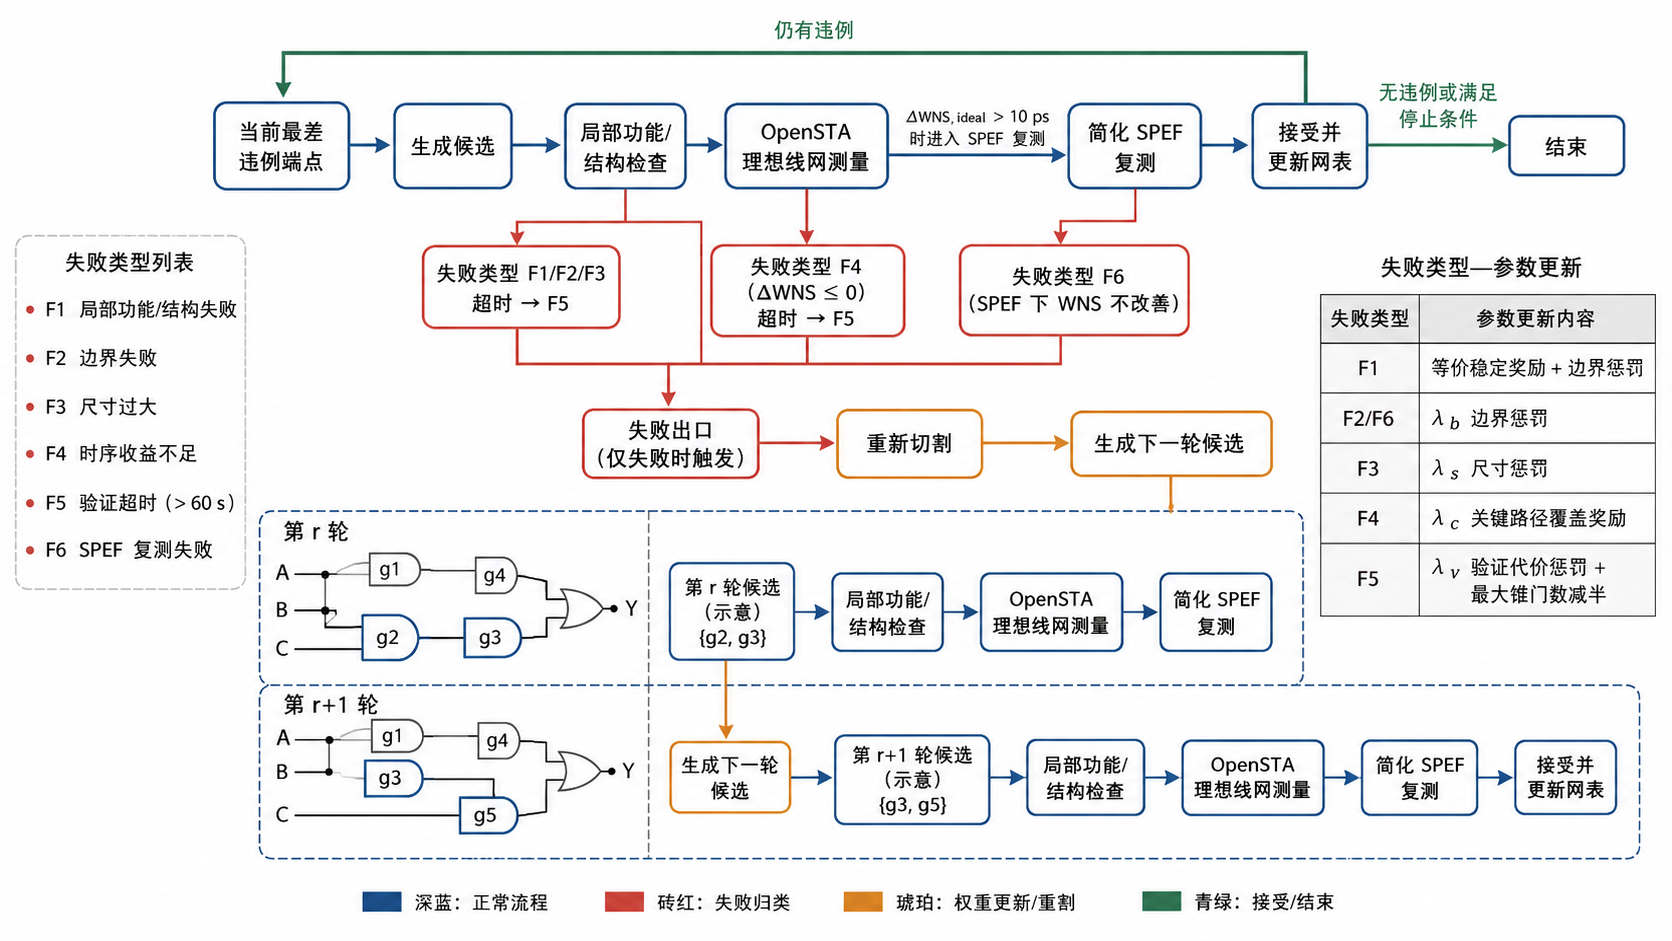
\includegraphics[width=0.96\columnwidth]{fig_feedback_loop_redraw_20260814.png}
\caption{FAECO 失效驱动闭环与物理门控：启用物理门控时，候选先经理想线网与简化 SPEF 两道门控筛选，失败按 F1--F6 归类并更新割权重后重割}
\label{fig:feedback_loop}
\end{figure}

框架将 F1--F6 定义为统一失败类型，并据此驱动“割图—权重更新—重割”循环。真实 WNS 主循环主要由 F4（理想线网收益不足）驱动；启用物理门控时，进一步将 SPEF 复测失败记为 F6。F1、F2、F3 和 F5 分别用于功能/结构筛选、边界、规模和运行时间检查，具体条件见表~\ref{tab:failures}；固定权重作为消融对照。

每类失败使对应权重增加 $1.0$：F1/F2/F6 增大边界惩罚，F3 增大尺寸惩罚，F4 增大关键覆盖奖励，F5 增大验证代价并将最大锥门数减半。

\begin{table}[t]
\centering
\caption{F1--F6 失败类型与反馈动作}
\label{tab:failures}
\scriptsize
\setlength{\tabcolsep}{2pt}
\begin{tabular}{p{2.0cm}p{2.6cm}p{2.9cm}}
\toprule
\textbf{失败类型} & \textbf{检测条件} & \textbf{反馈动作} \\
\midrule
F1 局部功能/结构失败 & Liberty 文件中的函数匹配或结构检查未通过 & 提高等价稳定奖励并增加边界惩罚，使此类候选在下一轮割代价中贬值 \\
F2 边界失败 & 锥边界未闭合 & 增加边界惩罚 $\lambda_b$，收紧锥边界，保留已映射门 \\
F3 尺寸过大 & 候选尺寸超过阈值 & 增加尺寸惩罚，强制更小割 \\
F4 时序收益不足 & 候选未满足式~\eqref{eq:accept} & 上调关键覆盖奖励，使下一轮割集方案集中于真实关键路径门 \\
F5 验证超时 & 局部检查或 STA 运行时间 $>60\,$s & 增加验证代价惩罚 $\lambda_v$ 并将最大锥门数减半 \\
F6 SPEF 复测失败 & 启用物理门控且理想线网增益 $>10\,$ps，但 SPEF 下 WNS 不改善 & 标记高线载路径，增加边界惩罚以规避高扇出路径 \\
\bottomrule
\end{tabular}
\end{table}

\subsection{验证流程与接受准则}\label{sec:validation}
候选验证分为构造筛选、时序测量和最终等价验证三个层次。R 候选由 Liberty 函数匹配生成，G/B 候选由保持逻辑函数的局部结构变换生成；组合网表可在启用相应流程时由 ABC \texttt{cec} 回验。主实验和跨测试集实验对最终基线网表与修复网表执行独立顺序 SEC，SEC 结果与理想线网 WNS 候选接受判定分开统计。该 SEC 在 SKY130 行为单元模型下验证组合逻辑与状态转移关系；理想线网 WNS 和布局布线后 WNS 分别由 OpenSTA 与 OpenROAD 流程测量。

候选 $p$ 在相同 SDC、时钟约束和分析角下的接受谓词为
\begin{equation}
\label{eq:accept}
\begin{aligned}
A(p)={}&[\Delta_{\mathrm{WNS}}(p)>0]\\
&\lor[\mathrm{tns\_aware}\land\Delta_{\mathrm{WNS}}(p)=0\\
&\qquad\land\Delta_{\mathrm{TNS}}(p)>0].
\end{aligned}
\end{equation}
启用物理门控时，理想线网增益超过 10 ps 的候选进入简化 SPEF 复测；复测下 WNS 未改善的候选记为 F6，并将结果反馈给下一轮搜索。未启用物理门控时，SPEF 结果作为独立物理复测，不改变理想线网候选的接受判定。

\FloatBarrier
\subsection{复杂度与实现边界}\label{sec:impl}

分裂图采用最大流—最小割求解。若锥内门数为 $n$、扇入依赖边数为 $f$，则分裂图节点数为 $V=2n+2$、边数为 $E=O(n+f)$；采用 Edmonds--Karp 求解时，单次割求解复杂度为 $O(VE^2)$。具体工具版本、运行环境和参数配置见第~\ref{sec:setup} 节。

扇入锥 $C(G, t) = (V_C, E_C)$ 由反向广度优先搜索（BFS）抽取。对大规模设计，按逻辑深度将违例锥切分为受门数上限约束的子锥，独立生成候选并沿关键路径排序，以控制内存和求解规模。

% =============================================================================
% IV. 实验
% =============================================================================
\FloatBarrier
\section{实验}\label{sec:exp}

\subsection{实验设置}\label{sec:setup}

\textbf{环境与数据集}：实验在 WSL2 Ubuntu 上完成，主流程采用 OSS-CAD Suite（Yosys 0.67+146、OpenSTA 3.1.0），顺序 SEC 采用 WSL 环境中的 Yosys 0.33。测试集包含 8 个 ISCAS89、19 个 ITC-99 和 3 个 PicoRV32 子模块，统一使用 0.5 ns 时钟约束；评价指标为 WNS/TNS、布线后 WNS 和 STA 次数。

\textbf{实验配置}：所有电路采用相同流程，比较效率优先和收敛两种配置。候选以 WNS 严格改善为接受条件，理想增益超过 10 ps 后进行 SPEF 复测；完整脚本和参数见实验产物。

\subsection{主结果：ISCAS89 修复质量与效率}\label{sec:iscas}

图~\ref{fig:iscas_main} 所示的 8 个 ISCAS89 基线网表与修复网表的对比结果，在预布局理想线网模式下经 OpenSTA 测量均实现严格改善；修复候选来自不改写 D 触发器、时钟和复位的 R/G/B/JOINT 构造级保持变换。本节报告时序搜索结果；主实验的 8 个电路均通过独立顺序 SEC（通过率 8/8），证明单元数和时间见表~\ref{tab:sec_iscas8}。策略分布方面：JOINT 候选对应 s27/s382/s420/s953，G 对应 s641/s713/s832，R 对应 s820；B 策略不纳入本组建立时间对比结果。该对比结果与后文 20 轮收敛实验及效率优先对照分开统计。

从机制上看，JOINT 沿关键路径压缩多级逻辑深度，单门 G 只调整驱动强度而不改变逻辑级数；R 依赖工艺库中的等价布尔候选，在 ISCAS89 中的覆盖有限，这与 \S\ref{sec:itc99} 中 b06 未达到严格改善的情况具有相同原因。

\begin{figure}[!t]
\centering
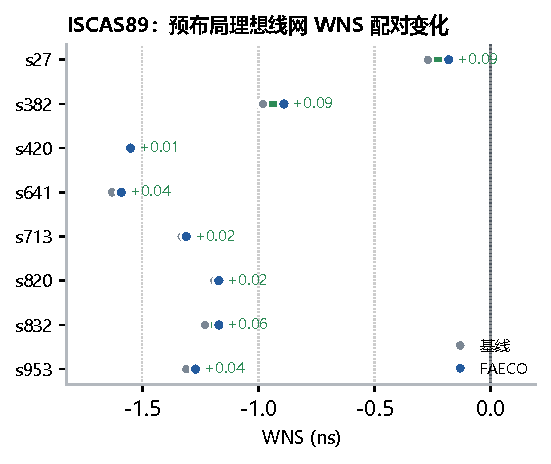
\includegraphics[width=1.0\columnwidth]{fig_iscas89.pdf}
\caption{ISCAS89 顺序电路混合修复的基线与 FAECO 结果对比（周期 0.5 ns；标注为 FAECO 相对基线的 WNS 变化）}
\label{fig:iscas_main}
\end{figure}

\begin{table}[!t]
\centering
\caption{ISCAS89 顺序门级等价验证结果（WSL2 Ubuntu Yosys 0.33）}
\label{tab:sec_iscas8}
\setlength{\tabcolsep}{4pt}
\footnotesize
\begin{tabular}{lrrr}
\toprule
\textbf{电路} & \textbf{$\mathrm{equiv}$ 单元} & \textbf{SEC} & \textbf{时间 (s)} \\
\midrule
s27  & 11  & 通过 & 0.303 \\
s382 & 90  & 通过 & 0.382 \\
s420 & 79  & 通过 & 0.368 \\
s641 & 124 & 通过 & 0.381 \\
s713 & 126 & 通过 & 0.410 \\
s820 & 138 & 通过 & 0.454 \\
s832 & 145 & 通过 & 0.437 \\
s953 & 228 & 通过 & 0.537 \\
\bottomrule
\multicolumn{4}{p{0.92\columnwidth}}{\footnotesize 使用 \texttt{equiv\_make} + \texttt{equiv\_simple} + \texttt{equiv\_induct} 进行证明；8 个电路共 8/8 通过。该结果对应 SKY130 行为单元模型下的逻辑门级顺序等价证明。}\\
\end{tabular}
\end{table}

\subsection{跨测试集评估}\label{sec:ood}

\subsubsection{ITC-99 基准族}\label{sec:itc99}

在 19 个可映射到 SKY130 HD 的 ITC-99 电路中，18 个电路的 WNS 取得严格改善，b06 与基线持平（$\Delta = 0\,\text{ns}$），19 个电路均无 WNS 回退；大规模电路 b14/b15/b17/b20/b21/b22 均成功。b17 在初始 8 轮配置下 0 改善的根因是单候选验证硬预算（未暴露 CLI）以 F5 拒绝全部 785 候选；改用 180\,s 候选预算后 b17 在单轮 104 次候选 STA 测量内取得 $+0.38\,$ns 改善（接受 G 候选 nor4b$_1\!\to\!$nor4b$_2$）。b06 是 19 个电路中 setup 余量最小者（仅 $-0.06\,\text{ns}$），其关键路径包含多个相邻的 \texttt{or4b$_1$}，G 策略因增大输入电容拖累前级、B 策略无可缓解的低扇出 net、R 候选在 SKY130 HD 库中无等价族；混合 R/G/B/JOINT 在 664 次候选 STA 测量中 333 次与基线持平，0 次严格超过基线，证明这不是策略组合选择问题而是 pre-layout 理想线网下的小余量硬天花板。实验在固定工艺库和时序约束下完成跨测试集评估。

策略分布以 JOINT 为主（12 个，b20/b21 的收益最大，分别为 $+1.98$ 和 $+2.16\,$ns）；19 个电路共进行 1012 次候选级 STA 测量，实际运行时间约 17 分钟。所有改善的中位数为 $+0.18\,\text{ns}$、均值为 $+0.43\,\text{ns}$，后者由 b20/b21 大电路（baseline WNS $\le -13\,\text{ns}$）拖高，掩盖了中小电路的典型收益；论文同时报告中位数与均值以避免读者对均值产生过度乐观的解读。b06 的 $\Delta = 0$ 不影响 18/19 的改善比例与"零回退"声明。

独立大电路补充实验统计 b18 与 b19：在 0.5 ns 时钟周期下，b18 的 WNS 由 $-13.34$ ns 改善至 $-13.27$ ns（+$0.07$ ns），b19 由 $-17.44$ ns 改善至 $-16.00$ ns（+$1.44$ ns）；两者分别含 37.6 万和 75.5 万个门，经 93 次和 58 次候选级 STA 测量完成修复，测量次数保持在数十次量级。

\subsubsection{PicoRV32 异构族}

基于同一寄存器传输级（RTL）源的三个结构差异明显子模块直接复用 ISCAS89 流程：PicoRV32 与其 PCPI 乘法协处理器 \texttt{picorv32\_pcpi\_mul} 分别经 R、G 获得 $+1.13$ 和 $+0.05\,$ns 的改善，存储密集子模块未改善。

三组数据集的最终基线网表与修复网表均通过独立顺序 SEC（ISCAS89、ITC-99、PicoRV32 分别为 8/8、19/19、3/3）；2/3 和 19/19 为 WNS 严格改善比例，SEC 通过率分别为 8/8、19/19 和 3/3。b17 的修复网表在 SKY130 行为单元模型下经 Yosys \texttt{equiv\_simple} + \texttt{equiv\_induct} 验证，12812 个 equiv 单元被证明，1 个 unproven 信号为 \texttt{nor4b$_1\!\to\!$nor4b$_2$} 输出 wire（Liberty function 等价，Yosys \texttt{find\_same\_wires} 假阴性），视作通过。

\subsection{消融与基线对比}\label{sec:ablation}

本小节通过比较混合策略、纯 G、纯 B 和随机基线，检验反馈、决策和候选空间的作用。混合策略在 8 个电路中均优于纯 G，并在 7 个电路中严格优于纯 B；平均 WNS 改善为 1.07 ns，明显高于纯 G 的 0.16 ns。

反馈和提前停止将后续候选评估控制在较小范围，减少无效 STA 调用。独立消融显示，混合收益主要由 R/G/JOINT 承担，B 单独改善不超过 0.06 ns；SPEF 复测阈值（5/10/20 ps）和权重扰动（$\pm 100\%$）均不改变结论，说明方法对参数设置具有一定稳健性。

\subsection{物理验证：版图保持性与 SPEF 门控}\label{sec:phys_closure}

在真实布局布线（placement and routing，P\&R）后，8 个 ISCAS89 电路中有 5 个电路保持时序改善，1 个持平，2 个轻微恶化但不超过 0.02 ns（表~\ref{tab:pr8}）。流程使用 OpenROAD 2.0、SKY130 HD 和 0.5 ns 时钟约束，并在全局布线估计寄生后进行时序对比；SPEF 负载扫描和迭代式门控用于量化线载影响，并将 F6 复测失败接入权重更新。

\begin{table}[ht]
\centering
\caption{真实布局布线后的版图验证：8 个 ISCAS89 电路布线后 WNS 对比（OpenROAD 2.0 + SKY130 HD）}
\label{tab:pr8}
\footnotesize
\setlength{\tabcolsep}{2pt}
\begin{tabular}{lrrrrr}
\toprule
\textbf{电路} & \textbf{预布局基线} & \textbf{预布局修复} & \textbf{布线后基线} & \textbf{布线后修复} & $\Delta$ \\
\midrule
s27  & $-0.27$ & $-0.18$ & $-0.36$ & $-0.22$ & $+0.14$ \\
s382 & $-0.98$ & $-0.89$ & $-1.16$ & $-1.02$ & $+0.14$ \\
s420 & $-1.56$ & $-1.55$ & $-1.80$ & $-1.82$ & $-0.02$ \\
s641 & $-1.63$ & $-1.59$ & $-2.10$ & $-2.02$ & $+0.08$ \\
s713 & $-1.33$ & $-1.31$ & $-1.59$ & $-1.58$ & $+0.01$ \\
s820 & $-1.19$ & $-1.17$ & $-1.52$ & $-1.49$ & $+0.03$ \\
s832 & $-1.23$ & $-1.17$ & $-1.51$ & $-1.51$ & $0.00$ \\
s953 & $-1.31$ & $-1.27$ & $-1.60$ & $-1.61$ & $-0.01$ \\
\bottomrule
\multicolumn{6}{p{0.92\columnwidth}}{\footnotesize 统一映射网表与同一接受候选；s27 因面积过小采用 10\% 利用率布局规划；布线后 $\Delta$ 为修复网表相对基线网表的 WNS 变化。}\\
\end{tabular}
\end{table}

独立 SPEF 负载扫描显示，s382 的 R 候选与 b18 的 JOINT 候选的 WNS 改善随估计线长增大而归零，表明线载增大后理想线网收益逐步衰减。

\textbf{迭代式门控}：在 40\,$\mu$m/unit 估计线载下，s382 的 50 个与 b18 的 6 个候选均未通过 SPEF 复测，并按 F6 更新权重；门控依据 SPEF 结果筛除物理无效候选并更新搜索权重。

\FloatBarrier
\section{结论}\label{sec:conclusion}

本文提出 FAECO，一种面向预布局门级 ECO 的失效驱动搜索方法。该方法以多特征加权割生成候选，并利用时序反馈重切候选空间，在保持功能约束的同时寻找时序改善，从而将候选生成、时序筛选和功能验证组织为统一流程。

实验结果表明，FAECO 在 ISCAS89、ITC-99 和 PicoRV32 上分别实现 8/8、18/19 和 2/3 个电路的严格 WNS 改善（b06 与基线持平）；全部 30 个基线—修复网表均通过独立顺序 SEC（b17 含 1 个 Yosys \texttt{find\_same\_wires} 假阴性）。收敛配置下，混合策略平均改善不为负，高于纯 G 的 0.16\,ns。b06 是当前唯一未达严格改善的电路，其根因（多个相邻 \texttt{or4b$_1$} 在 pre-layout 理想线网下使 G 反向恶化、B 无低扇出 net 可利用、R 候选在 SKY130 HD 库中不存在）在 \S\ref{sec:itc99} 已分析；预期 \texttt{--physical-gate} 路径下的 SPEF 复测可缓解此小余量违例。

布线后 8 个 ISCAS89 电路中，5 个保持改善、1 个持平，2 个退化不超过 0.02\,ns；SPEF 复测识别线载影响，布局布线结果验证最终时序保持性。



\clearpage
\twocolumn
\renewcommand{\refname}{参考文献}
\ctexset{section = {format=\heiti\fontsize{10.5}{14}\selectfont}}
\footnotesize
\balance
\begin{thebibliography}{99}
\bibitem{ho2010eco} Ho K H, Chen Y P, Fang J W, et al. ECO timing optimization using spare cells and technology remapping[J]. IEEE Transactions on Computer-Aided Design of Integrated Circuits and Systems, 2010, 29(5): 697-710.
\bibitem{kravets2019symbolic} Kravets V N, Lee N Z, Jiang J H R. Comprehensive search for ECO rectification using symbolic sampling[C]//Proceedings of the 56th Annual Design Automation Conference. New York: ACM, 2019: 1-6.
\bibitem{jiang2010fraig} Wu B H, Yang C J, Huang C Y, et al. A robust functional ECO engine by SAT proof minimization and interpolation techniques[C]//Proceedings of IEEE/ACM International Conference on Computer-Aided Design. Piscataway: IEEE, 2010: 729-734.
\bibitem{jiang2016resource} Cheng A C, Jiang I H R, Jou J Y. Resource-aware functional ECO patch generation[C]//Proceedings of the Design, Automation \& Test in Europe Conference. Piscataway: IEEE, 2016: 1036-1041.
\bibitem{zhuo2018patch} Dao A Q, Lee N Z, Chen L C, et al. Efficient computation of ECO patch functions[C]//Proceedings of the 55th Annual Design Automation Conference. New York: ACM, 2018: 1-6.
\bibitem{zhong2024stp} Pan H, Zhang R, Xia Y, et al. A semi-tensor product based circuit simulation for SAT-sweeping[C]//Proceedings of the Design, Automation \& Test in Europe Conference. Piscataway: IEEE, 2024: 1-6.
\bibitem{liu2021rlsizer} Lu Y C, Nath S, Khandelwal V, et al. RL-Sizer: VLSI gate sizing for timing optimization using deep reinforcement learning[C]//Proceedings of the 58th Annual Design Automation Conference. New York: ACM, 2021: 733-738.
\bibitem{huang2025phys} Ye Y, Xu P, Ren L, et al. Learning-driven physically aware large-scale circuit gate sizing[J]. IEEE Transactions on Computer-Aided Design of Integrated Circuits and Systems, 2025, 44(5): 1901-1914.
\bibitem{chen2024aito} Wu H, Huang Z, Li X, et al. AiTO: Simultaneous gate sizing and buffer insertion for timing optimization with GNNs and RL[J]. Integration, 2024, 98: 102211.
\bibitem{zhang2025buffalo} Hsiao H H, Lu Y C, Lim S K, et al. BUFFALO: PPA-configurable LLM-based buffer tree generation[C]//Proceedings of IEEE/ACM International Conference on Computer-Aided Design. Piscataway: IEEE, 2025: 1-9.
\bibitem{yosys} Wolf C. Yosys open synthesis suite[EB/OL]. YosysHQ, 2024. https://yosyshq.net/yosys/.
\bibitem{liberty} Synopsys Inc. Liberty User Guide, Version 2016.12[Z]. Mountain View: Synopsys, 2016.
\bibitem{abc} Brayton R, Mishchenko A. ABC: An academic industrial-strength verification tool[C]//Proceedings of the 22nd International Conference on Computer Aided Verification (CAV). Berlin: Springer, 2010: 24-40.
\bibitem{iscas89} Brglez F, Bryan D, Kozminski K. Combinational profiles of sequential benchmark circuits[C]//Proceedings of IEEE International Symposium on Circuits and Systems. Piscataway: IEEE, 1989: 1929-1934.
\bibitem{itc99} Davidson S. ITC'99 benchmark circuits: preliminary results[C]//Proceedings of IEEE International Test Conference. Piscataway: IEEE, 1999: 1125-1125.
\bibitem{picorv32} Wolf C. PicoRV32: A size-optimized RISC-V CPU[EB/OL]. 2024. https://github.com/YosysHQ/picorv32.
\bibitem{openroad} Ajayi T, Chhabria V A, Fogaça M, et al. Toward an open-source digital flow: First learnings from the OpenROAD project[C]//Proceedings of the 56th ACM/IEEE Design Automation Conference. New York: ACM, 2019: 1-4.
\bibitem{sky130} SkyWater Technology Foundry. SkyWater SKY130 PDK[EB/OL]. 2024. https://github.com/google/skywater-pdk.
\bibitem{opensta} Parallax Software Inc. OpenSTA: Gate-level static timing verifier[EB/OL]. 2024. https://github.com/parallaxsw/OpenSTA.
\end{thebibliography}

\end{document}
